% =============================================================================
%  Figure: deployment + instrumentation template (one connector, one arm)
%  ---------------------------------------------------------------------------
%  Standalone-compilable:  pdflatex deployment-topology.tex
%  Compiled PDF is included in the thesis as figures/deployment-topology.pdf.
%  Style matches figures/src/identity-onoff-parity.tex (grayscale, lmodern).
%  Solid arrows = pushed (requests, telemetry); dashed arrows = pulled/queried.
% =============================================================================
\documentclass[border=6pt]{standalone}
\usepackage{lmodern}
\usepackage{tikz}
\usetikzlibrary{positioning, calc, arrows.meta}

\begin{document}
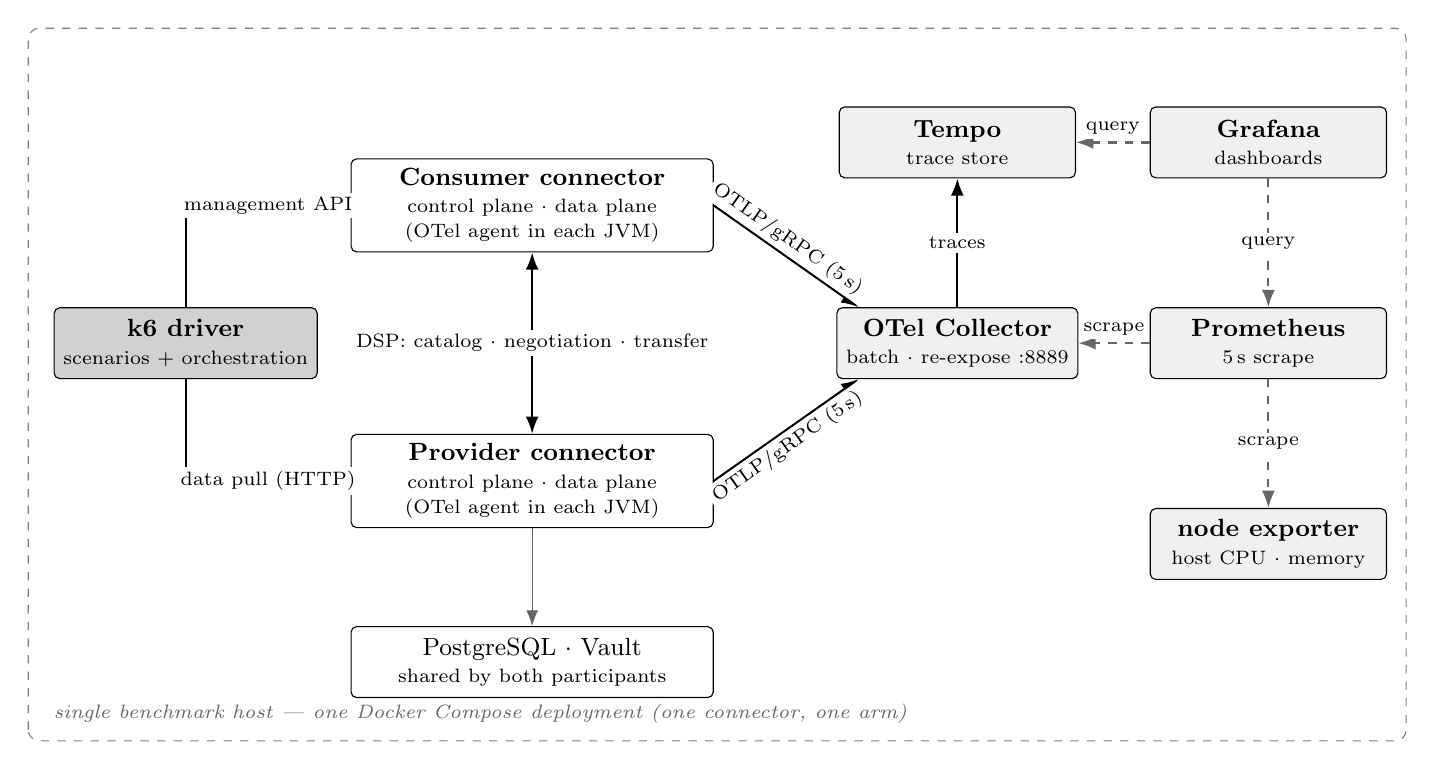
\begin{tikzpicture}[
  box/.style     = {draw, rounded corners=2pt, align=center, font=\small,
                    fill=white, minimum height=0.9cm},
  sut/.style     = {box, minimum width=4.6cm},
  mon/.style     = {box, fill=black!6, minimum width=3.0cm},
  drv/.style     = {box, fill=black!18, minimum width=2.9cm},
  arr/.style     = {-{Latex[length=2.2mm]}, thick},
  thin/.style    = {-{Latex[length=2mm]}, draw=black!60},
  pull/.style    = {-{Latex[length=2.2mm]}, thick, dashed, draw=black!60},
  lbl/.style     = {font=\scriptsize, fill=white, inner sep=1.5pt},
]

% ---- host boundary ----------------------------------------------------------
\draw[rounded corners=4pt, dashed, draw=black!50]
  (-8.6,-4.7) rectangle (8.9,4.35);
\node[anchor=south west, font=\scriptsize\itshape, text=black!60] at (-8.4,-4.6)
  {single benchmark host --- one Docker Compose deployment (one connector, one arm)};

% ---- load driver (left) -----------------------------------------------------
\node[drv] (k6) at (-6.6,0.35)
  {\textbf{k6 driver}\\[-1pt]\scriptsize scenarios + orchestration};

% ---- systems under test (middle) --------------------------------------------
\node[sut] (cons) at (-2.2,2.1)
  {\textbf{Consumer connector}\\[-1pt]
   \scriptsize control plane $\cdot$ data plane\\[-2pt]
   \scriptsize (OTel agent in each JVM)};
\node[sut] (prov) at (-2.2,-1.4)
  {\textbf{Provider connector}\\[-1pt]
   \scriptsize control plane $\cdot$ data plane\\[-2pt]
   \scriptsize (OTel agent in each JVM)};
\node[sut] (db) at (-2.2,-3.7)
  {PostgreSQL $\cdot$ Vault\\[-1pt]\scriptsize shared by both participants};

% driver -> consumer management API, driver -> provider data pull
\draw[arr] (k6.north) |- node[lbl, pos=0.75] {management API} (cons.west);
\draw[arr] (k6.south) |- node[lbl, pos=0.75] {data pull (HTTP)} (prov.west);
% DSP between the participants
\draw[arr, {Latex[length=2.2mm]}-{Latex[length=2.2mm]}] (cons.south) --
  node[lbl] {DSP: catalog $\cdot$ negotiation $\cdot$ transfer} (prov.north);
% persistence
\draw[thin] (prov.south) -- (db.north);

% ---- observability plane (right) --------------------------------------------
\node[mon] (col) at (3.2,0.35)
  {\textbf{OTel Collector}\\[-1pt]\scriptsize batch $\cdot$ re-expose :8889};
\node[mon] (tempo) at (3.2,2.9)
  {\textbf{Tempo}\\[-1pt]\scriptsize trace store};
\node[mon] (prom) at (7.15,0.35)
  {\textbf{Prometheus}\\[-1pt]\scriptsize 5\,s scrape};
\node[mon] (nodex) at (7.15,-2.2)
  {\textbf{node exporter}\\[-1pt]\scriptsize host CPU $\cdot$ memory};
\node[mon] (graf) at (7.15,2.9)
  {\textbf{Grafana}\\[-1pt]\scriptsize dashboards};

% agents push OTLP to the collector
\draw[arr] (cons.east) -- node[lbl, sloped, above, pos=0.45] {OTLP/gRPC (5\,s)} (col.160);
\draw[arr] (prov.east) -- node[lbl, sloped, below, pos=0.45] {OTLP/gRPC (5\,s)} (col.200);
% collector -> tempo (traces)
\draw[arr] (col.north) -- node[lbl] {traces} (tempo.south);
% prometheus pulls
\draw[pull] (prom.west) -- node[lbl, above=1pt] {scrape} (col.east);
\draw[pull] (prom.south) -- node[lbl] {scrape} (nodex.north);
% grafana queries
\draw[pull] (graf.south) -- node[lbl] {query} (prom.north);
\draw[pull] (graf.west) -- node[lbl, above=1pt] {query} (tempo.east);

\end{tikzpicture}
\end{document}
